\documentclass[12pt]{report}
\usepackage[T1]{fontenc}
\usepackage[utf8]{inputenc}
\usepackage{graphicx}
\usepackage{amsmath,amsfonts}
\usepackage{newtxtext,newtxmath}
\usepackage{url}
\usepackage{fixltx2e}
\usepackage{minted}
\usepackage{xcolor}

% \usepackage{parskip}

%\usepackage[polish]{babel}

\renewcommand{\chaptername}{Chapter}
\renewcommand{\contentsname}{Table of contents}
\renewcommand{\figurename}{Fig.}
\renewcommand{\tablename}{Tab.}
\renewcommand{\listfigurename}{List of figures}
\renewcommand{\listtablename}{List of tables}
\renewcommand{\bibname}{Bibliography}

\renewcommand{\labelitemi}{$\diamond$}

\pagestyle{headings}

\setlength{\textwidth}{14cm}
\setlength{\textheight}{20cm}

% \setlength{\parindent}{20pt}

\newtheorem{definition}{Definition} % przykład nowego środowiska 
\newtheorem{example}{Example}[chapter] % przykład nowego środowiska 
\newtheorem{corollary}{Corollary}[chapter] % przykład nowego środowiska [corollary => wniosek] 



\begin{document}
\tableofcontents	% generuje spis treści ze stronami !!!

%\indent - wymuszony odstep
%\bf - pogrubienie

\chapter{Introduction} \label{rozdz.wstep} 
In the age of ubiquitous Internet access more and more human activities take place in the Web. E-commerce, the act of shopping online, has been on the increase for many years. [{\bf tutaj jakies statystyki, dane nt udzialu ecommerce w ogolnej sprzedazy}]

The amount of products offered on the Internet can be overwhelming for an average consumer, therefore companies take efforts to properly target users with relevant content. Correct product targeting directly translates to increased sales. [{\bf jakis reference}] Systems responsible for this are {\bf recommender systems}.

In the last several years the world has witnessed the rise of social media - Internet-based applications enabling users to connect with each other and share various content. The principal services include Facebook, Twitter and LinkedIn. This phenomenon enabled large-scale user information gathering. That information can be shared with third parties (with user consent) and can be used by them to improve user experience. [{\bf doszlifowac}]

The use of social media in e-commerce is commonly referred to as {\bf social commerce}. According to Lora Cecere of Altimeter Group \cite{rise_of_social_commerce}, "Social Commerce is the use of Social Technologies to connect, listen, understand and engage to improve the shopping experience."

% The aim of this thesis is to create a recommender system that leverages user social media information to suggest products. The implementation will be a demo web e-commerce store.[{\bf rozwinac?}]


% Tutaj ogólnie w skrócie o wzroście znaczenia ecommerce, social commerce etc.
% Coraj więcej produktów, czasem trudno się w tym odnaleźć.
% Rekomendacje dobre zarówno dla klientów (szybciej mogą znaleźć to, czego potrzebują), jak i dla sklepów (większe zyski).

\section{Scope of work}
The thesis involves the areas of software engineering, web development, systems integration and recommender systems.

The aim of this thesis is to design and create a recommender system that leverages users' social media information to suggest products. 

While there exist many recommender systems, most of them require initial information about user preferences regarding some part of data that the later recommended items come from. For example, if a user is to be recommended a movie to watch, the system needs either a history of movies the user has seen, his ratings on multiple movies etc. [{\bf dopracowac}] Next, this information can be processed in two ways:
\begin{itemize}
\item collaborative filtering - based on item ratings, other users with similar tastes are found and items they like are proposed
\item content-based filtering - based on item ratings, items similar to the highest ranked items are found and proposed
\end{itemize}



Są już systemy rekomendacyjne, ale cierpią na 2 główne problemy: cold start i data sparsity. Tu można zaczerpnąć z \cite{snrs}, pp.1-2. 
Wykorzystanie grafowej bazy danych, dobrze modelującej relacje społeczne.

Osoba podejmująca tematykę stoi przed wyzwaniami: zbudować rzetelną bazę produktów, bazę użytkowników, przekonać użytkowników do udostępnienia danych osobowych etc.

Spodziewane efekty:\\
- rzetelne rekomendacje tuż po zalogowaniu użytkownika\\
- ...\\

% Dlaczego podejmowanie tej tematyki jest potrzebne? Czy są inne
% rozwiązania tego problemu/tych problemów? Jakie? czy są lepsze/gorsze,
% tańsze/droższe, itp.
% \indent Przed jakimi wyzwaniami stoi osoba podejmująca tematykę? \\
% \indent {\bf Określić spodziewane efekty pracy:} W wyniku doświadczeń przeprowadzonych w zakresie pracy polepszeniu
% uległo.... podać konkretne wskaźniki rezultaty, jak np. przyspieszenie obliczeń,
% redukcja kosztu, nowe oprogramowanie itp. w złotówkach, sekundach, procentach,
% roboczogodzinach itp. 

% {\bf (razem max. 3 strony - strona przeliczeniowa = 1800 znaków, średnio 30
% wierszy po 60 znaków)}

\section{Objectives}

- ofkors że zrobić RS [rozwinąć to]

- zaimplementować jako stronkę
    -- ma być "ładna", żeby testowi userzy chcieli wypełnić ankietę

% Wymienić w punktach cele pracy, rozpoczynając od celów poznawczych (dotyczą\-cych
% zebrania wiadomości, przybliżenia/popularyzacji technik / metod / zagaadnień).
% W~drugiej kolejności wyienić cele praktyczne.
% \subsubsection{Przybliżenie (popularyzacja) metody/technologii/systemu...}
% \subsubsection{Propozycja rozwiązania problemu....}
% \subsubsection{Opis zastosowania technologii X w problemie Y...}
% \subsubsection{Przedstawienie prototypu systemu/układu/aplikacji...}
% \subsubsection{Określenie przydatności algorytmu Z do rozwiązania problemu T.....
% }
% \subsubsection{Opracowanie strategii ... w celu poprawy wydajności/jakości...}
% \subsubsection{Ocena możliwości wdrożenia proponowanych rozwiązań, ich wartość
% praktyczna, lokalne i globalne możliwości zastosowania}
% \subsubsection{itp.}

% Każdy cel opisać w minimum 2-3 zdaniach. Użyte określenia muszą być powszechnie
% zrozumiałe, nie stosujemy skrótów, slangu,  tzw. makaronizmów, np. ,,softłer''.
% {\bf cały podrozdział ok. 1 strony przeliczeniowej czyli 1800 znaków}

\section{Research method}
% \begin{itemize}
% \item Studia literaturowe
% \item Analiza budowy i działania istniejących produktów
% \item Projektowanie i prototypowanie nowatorskich rozwiązań 
% \item Obliczenia i ........
% \end{itemize}

% Każdy element opisać w minimum 2-3 zdaniach. Np. studia literaturowe powinny
% odnosić się do charakterystyki wykorzystanych źródeł książkowych, czyli: Jaka
% jest podstawowa literatura dziedziny, czy jest dostępna w języku polskim, czy trzeba je tłumaczyć, czy wiedza na ten
% temat jest zebrana w jednym miejscu, czy jej synteza jest osobnym zadaniem itp. 
% Jak duży jest udział źródeł elektronicznych w tej ,,działce'' wiedzy i badań,
% itd. \\
% \indent Jakie metody badawcze są typowe dla danego tematu. Dlaczego je
% zastosowano, ewentualnie dlaczego zastosowano inne? \\
% WYMAGANE ODNOŚNIKI DO POZYCJI BILIOGRAFII.\\
% {\bf cały podrozdział ok. 1 strony przeliczeniowej czyli 1800 znaków}.

\section{Literature overview} % ?? czy to będzie ?
% Rozszerzyć odpowiedni podpunkt z metody badawczej, np. wg podziału:
% \subsubsection{Źródła książkowe polskojęzyczne i tłumaczenia}
% \subsubsection{Źródła książkowe obcojęzyczne}
% \subsubsection{Artykuły naukowe, raporty z badań, komunikaty konferencyjne,
% dokumentacje techniczne, manuale, instrukcje}
% \subsubsection{Źródła elektroniczne}


\section{Thesis plan}
% Tematem pracy jest: ....., zaś za główny cel przyjęto ...... . \\
% Rozdział \label{rozdz.wstep} zawiera wstęp i cele pracy. W rozdziale drugim
% opisano/...... w Rozdziale 3. zawarto............ Rozdział 4. przedstawia..... \\
% W podsumowaniu pracy przedstawiono..........................., z czego wynika,
% że ................  \\
% Najważniejszym wnioskiem/wynikiem/rezultatem pracy jest..................\\ {\bf wyraźnie określić
% CO TO JEST}. \\

% {\bf cały podrozdział ok. 1 strony}.




\chapter[Fundamental information on social...]{Fundamental information on social commerce, recommendation algorithms and graph databases} \label{fundamental_info}

\section{Social Commerce}

- opisać social media?\\
- opisać e-commerce?\\

Social commerce is the fusion of social media with e-commerce \cite{social_commerce_syzygy}. It uses social media, which are founded on user interactions and contributions, to improve the shopping experience on the Internet.

The term itself was created by Yahoo! in 2005, referring to an online place where people can share opinions and experiences, find products and services and buy them. Nevertheless, the roots of such practices date back to 1995, when Amazon started encouraging customers to rate and review products they had purchased \cite{social_commerce_syzygy}.

In the recent years, however, the popularization of social media services such as Facebook or Twitter has given rise to new social commerce tools and opportunities. Examples include social media stores, i.e. storefronts present directly on the social media sites, or portable social graphs, which give access to users' data to third parties. It is the latter that will be of interest to us in the context of this thesis.

% There are various tools and approaches in social commerce. Examples include social shopping, where we can chat with friends

Social commerce can give businesses the following advantages \cite{social_commerce_syzygy}:
\begin{itemize}
\item social media monetization
\item e-commerce sales optimization
\item business model innovation
\end{itemize}

From the customer's point of view, the buying experience can be improved in the following ways \cite{social_commerce_syzygy}:
\begin{itemize}
\item product discovery (social commerce acts as an Awareness Booster)
\item product selection (Decision Accelerator)
\item product referral (Advocacy Activator)
\end{itemize}

According to Dr Paul Marsden of Syzygy Group \cite{social_commerce_syzygy}, there are six dimensions or toolsets for social commerce:
\begin{enumerate}
\item Social Shopping
\item Ratings and Reviews
\item Recommendations and Referrals
\item Forums and Communities
\item Social Media Optimization
\item Social Ads and Apps
\end{enumerate}

In this thesis I will focus only on the Recommendations approach to social commerce.

[TODO]

\section{Recommender Systems}

\subsection{Title?}

Recommender Systems (RSs) are software tools and techniques generating recommendations for items that might be interesting to a user \cite{rec_sys_handbook}. "Item" is a general term referring to what the system can recommend. It can be almost anything, from movies to watch, music to listen to, products to buy, news to read etc.

One category are the non-personalized recommendations. These typically are the "top" lists, such as "top 10 best rated movies", "top 50 most shopped products". They are simple and may provide a good starting point when no information about a user is known, however they are not in the scope of the RS research.

% It is the personalized recommendations that are tackled by RSs.
What the RSs deal with are personalized recommendations. They can be seen as ranked lists of items, most suitable for a user, based on his preferences. To create such a list, the RS requires either explicit user preferences, e.g. ratings of items, or implicit information, i.e. which products the user browsed, how long did they look at each product, what music have they listened to recently.

RSs are based on the observation that people tend to follow recommendations of others while making everyday decisions \cite{rec_sys_handbook}. Moreover, the second assumption is that if we have similar tastes to someone else, their recommendation would be more accurate than that of a random stranger.

[Functions of recommender systems? (\cite{rec_sys_handbook})]

\subsection{Recommendation Techniques}

In order to be able to suggest items, a RS must implement a way of predicting the utility of an item to the user. Typically this degree of utility of an item \textit{i} for the user \textit{u} is modelled as a function \textit{R(u,i)}. Then the RS has to predict the value of \textit{R} for each user-item pair - compute \textit{\^{R}(u,i)}, where \textit{\^{R}} is the estimation of the true function \textit{R}. Therefore, for each user, having calculated the prediction on a set of items, i.e., \textit{\^{R}(u,i\textsubscript{1}),...,\^{R}(u,i\textsubscript{N})} the system will recommend the items \textit{i\textsubscript{j\textsubscript{1}},...,i\textsubscript{j\textsubscript{K}}} ($K \leq N$) with the largest predicted utility \cite{rec_sys_handbook}.

The two most popular classes of recommender systems are {\bf content based} and {\bf collaborative filtering} RSs \cite{rec_sys_handbook}.

% \subsubsection{Content based}
\hbox{}
{\bf Content based:} The recommended items are similar to the ones that the user liked in the past. Similarities between items are calculated on the basis of their features, e.g. in the case of movies it can be their genre, actors, director etc.

The advantage of such an approach is that there is no need for other users in the system. It could work even if only a single user was using it.

However the disadvantage is that all items need to be well characterised by features, which imposes constraints on item addition. Moreover, only items of the same category can be compared, as it is impossible to directly compare features of, e.g. a movie and a music album. Therefore this kind of system could not work well in a multi-category environment.

% \subsubsection{Collaborative filtering}
\hbox{}
{\bf Collaborative filtering:} The idea is to recommend to the active user the items that other users with similar interests liked in the past. The similarity between two users is calculated on the basis of their past ratings of items. Then, if the RS finds that e.g. user B is most similar to the active user A, it will find items highly rated by B that A has not yet rated (thus probably does not know) and recommend them to user A.

This approach to RS allows for the items to be transparent to the system, i.e. it does not need to know what the items are nor what features, properties they have (as opposed to the content-based approach). It allows for greater flexibility when it comes to adding items.

The drawback is that in order for the system to work, it needs a large user base with ratings. Moreover, if a new item is added in the course of the system's functioning, it will be available for recommendations only after some users have rated it.

\hbox{}
There exist other types of recommender systems...

[TODO: opisać tutaj community-based (\cite{rec_sys_handbook}, p.13) jako podobny do mojego, ale bazujący tylko na znajomościach pobranych z SN, a nie na profilach użytkowników]

\subsection{Application}
[TODO: \cite{rec_sys_handbook}, p.14]

\section{Graph databases}

\subsection{Graphs}

A graph is a collection of vertices and edges, or, more simply put, a set of \textit{nodes} and the \textit{relationships} between them \cite{graph_databases}. It is a general purpose structure, where nodes represent entities and relationships - the ways these entities relate to each other.

Graph theory, the study of graph models and algorithms, has been used in many disciplines \cite{learning_neo4j}:
\begin{itemize}
\item {\bf Social studies}: Human beings are a social species, we are interconnected by relations. People interact with people every day, exchange items, ideas, therefore modelling those interactions with graphs seems natural.
\item {\bf Biological studies}: Biological components and their interactions can be modeled as a graph structure, which has many practical advantages.
\item {\bf Computer science}: The usage ranges from chip design, network management, recommendation systems, UML modeling to algorithm generation and dependency analysis.
\item {\bf Flow problems}: Used in telecom / gas / airline / package delivery networks to find the optimal path, bottlenecks, for capacity planning etc. 
\item {\bf Route problems}: To find the optimal route between two nodes on a network, e.g. car navigation systems.
\item {\bf Web search}: The original Google search algorithm, PageRank, was a graph algorithm.
\end{itemize}

[TODO więcej?]

\subsection{Graph Database Management Systems}

The main types of database management systems are:
\begin{itemize}
\item {\bf Relational databases}: Data is organized in tables of rows and columns. Because each row has a unique key, rows in a table can be linked to rows in other tables.
\item {\bf NoSQL databases}: The acronym standing for "Not Only SQL" represents a new generation of databases \cite{learning_neo4j}. These include:
\begin{itemize}
\item Key-Value stores
\item Column-Family stores
\item Document stores
\item Graph databases
\end{itemize}
\end{itemize}

A graph database management system is an online database management system with Create, Read, Update and Delete (CRUD) methods that expose a graph data model \cite{graph_databases}. Graph databases support transactions and are optimized in terms of transactional performance, integrity and operational availability.

When analyzing graph database technologies, it is important to consider the two factors \cite{graph_databases}:
\begin{itemize}
% \item {\bf Underlying storage}: 
% \item {\bf Processing engine}:
\item Underlying storage: Some graph databases use the so-called \textit{native graph storage}, designed solely for storing and managing graphs. Others, however, keep the data in other data stores, e.g. in a serialized form in a relational database.
\item Processing engine: The best performance is gained when a graph database implements \textit{native graph processing}, therefore the connected nodes physically point to each other in the database without the use of indices.
\end{itemize}

\begin{figure}[!t]
\centering
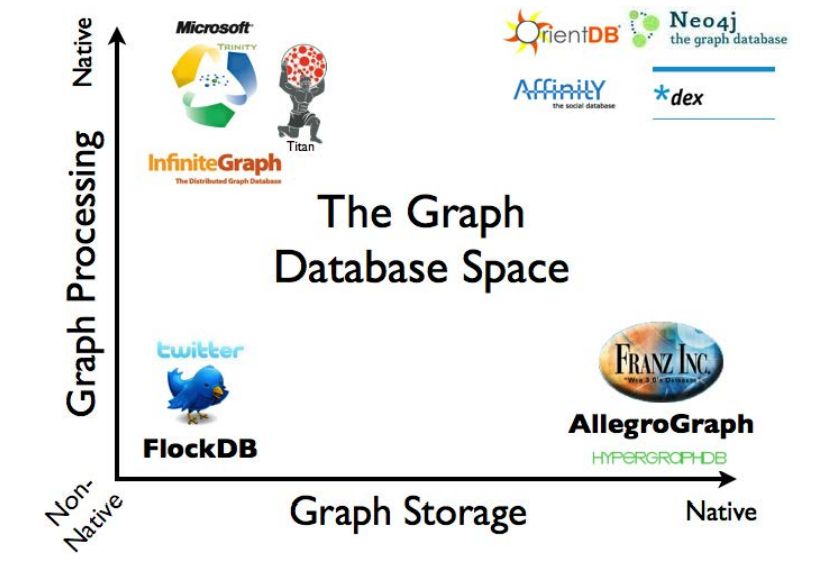
\includegraphics[width=\textwidth]{graph_databases_comp.jpg} 
\caption[Overview of graph databases.]{Overview of graph databases.\footnotemark{}}
\label{fig.graph_databases}
\end{figure}
\footnotetext{Image source: \cite{graph_databases}, p.7}

Figure \ref{fig.graph_databases} presents different graph database implementations in terms of their compliance with the nativity of both graph processing and graph storage. As it can be seen, Neo4j is one of the most advanced implementations in both aspects. Moreover it is very popular and well documented, therefore it was chosen as the graph database engine for this thesis.


\subsection{The Property Graph model}

Data is stored in a graph database using the Property Graph data model \cite{learning_neo4j}. In this model both nodes and relationships can have their \textit{properties}, represented by key--value pairs. It can be characterised by the following:
\begin{itemize}
\item There is no fixed schema.
\item The database can deal with semi-structured data, e.g. some nodes / relationships can have more or less properties than others and it causes no problems.
\item Nodes and their properties are analogous to rows in a table with fields.
\item Relationships are explicit, rather than established with a join operation at runtime. They can also have properties, which is unique as compared to relational databases.
\end{itemize}

Moreover, this data model was customized in Neo4j to allow for two additional important concepts:
\begin{itemize}
\item {\bf Node labels}: Each node can have one or more labels, which are a sort of a "special property". It helps create a type structure. They are useful for creating subgraphs in the database or to fetch only nodes of a specific type.
\item {\bf Relationship types}: Similar to node labels, but for relationships, however they are mandatory. Moreover each relationship can only have one type. They are useful for graph traversals limited to certain kinds of paths only.
\end{itemize}

\begin{figure}[!t]
\centering
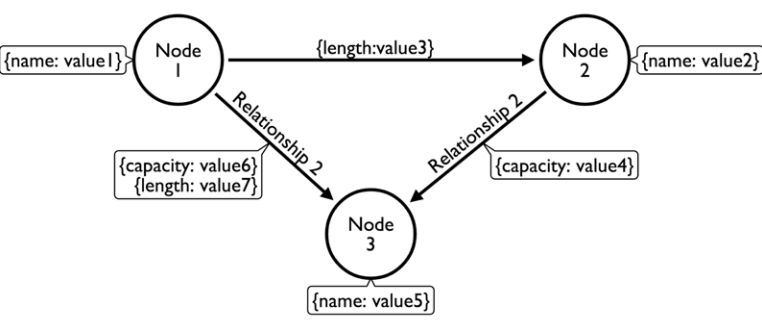
\includegraphics[width=\textwidth]{property_graph2.jpg} 
\caption[Property graph example.]{Property graph example.\footnotemark{}}
\label{fig.property_graph}
\end{figure}
\footnotetext{Image source: \cite{learning_neo4j}, p.35}

\subsection{Cypher Query Language}

Cypher is a declarative graph query language used to interact with the Neo4j database \cite{neo4j}. It is simple, yet can perform very complicated database queries. It focuses on \textit{what} to retrieve from a graph, not \textit{how} to do it, thus hiding the complexity from the user.

The structure of Cypher queries is similar to that of SQL. They are built up using various clauses that can be chained together and pass their result sets to the next ones.

The most basic clauses to read from the graph are:
\begin{itemize}
\item \texttt{MATCH}: The graph pattern to match.
\item \texttt{WHERE}: Adds constraints to a pattern.
\item \texttt{RETURN}: Defines what data to return from the query.
\end{itemize}

Clauses to update the graph:
\begin{itemize}
\item \texttt{CREATE} / \texttt{DELETE}: Create or delete nodes and relationships.
\item \texttt{SET} / \texttt{REMOVE}: Set values to or remove properties of nodes and relationships. 
\item \texttt{MERGE}: Match existing or create new nodes and patterns.
\end{itemize}

An example of a simple query is shown in Listing \ref{listing.cypher_sample1}. It returns all nodes with label \texttt{Vegetable} that the node with label \texttt{User} having the property "name" with value "Mike" is related to with the relationship type \texttt{LIKES}. In casual terms, it returns all vegetables that the user Mike likes.

\begin{listing}
\begin{minted}[framesep=3mm,fontsize=\footnotesize,bgcolor=gray!20]{psql}
MATCH (m:User {name:"Mike"})-[:LIKES]-(c:Vegetable)
RETURN c
\end{minted}
\caption{A sample Cypher query.}
\label{listing.cypher_sample1}
\end{listing}

\subsection{Comparison with relational and other NoSQL databases}

% Why use a graph database? \cite{learning_neo4j}, p.37

% [TODO Join bomb \cite{learning_neo4j}, p.27]

% ["graph databases actually take relational databases...", \cite{learning_neo4j}, p.33]

% [TODO The power of graph databases \cite{graph_databases}, p. 8]

Even though almost any dataset can be modelled as a graph, it does not mean it always should. There are many cases in which relational or other NoSQL databases are an equal or a better choice. For instance when dealing with large, set-oriented queries, which do not require a lot of joining or require a lot of aggregation on these sets, then the performance will be much better with a relational database. Similarly, with simple, aggregate-oriented queries a key--value or document store would be more efficient \cite{learning_neo4j}.

That said, there are certain scenarios where graph databases greatly outperform any other solutions \cite{learning_neo4j}. 
\begin{itemize}
\item {\bf Complex queries}: These are queries that involve a lot of join-style operations. They are very expensive operation in relational database system because of the need to compute the Cartesian product of the indices of tables that are being joined. In graph databases, however, these type of queries are pattern matching queries, which are performed by choosing a starting node and looking for matching occurrences of that pattern in the vicinity of that node - everything that is not connected to the starting node will be omitted. Therefore the performance does not depend on the dataset size, because usually everything is not connected to everything. 
\item {\bf Intensive queries on live data}: Typically in order to deeply analyze the relational data, it must be duplicated, denormalized and processed by techniques such as Extract, Transform and Load (ETL) to yield query-specific representations. This is because the performance on a live database would be too poor and could slow the entire database. Graph databases, however, are able to handle such complex queries between a web request and a web response, making it applicable to real-time analytics.
\item {\bf Path finding queries}: In graph databases, when looking for how two elements are interconnected, all that needs to be done is to apply a graph algorithm to a starting and an ending point. In the case of relational databases, one would have to explicitly state how to move from on table to another.
\end{itemize}

% \subsubsection{Performance}

% \subsubsection{Flexibility}

% \subsubsection{Agility}

\chapter[Presentation of existing social recommender...]{Presentation of existing social recommender systems}

\section{"A Social Network-Based Recommender System (SNRS)"}

In the paper \cite{snrs} the researchers from the University of California described their approach to creating a recommender system (RS) taking advantage of social data. They have created a system that incorporates the influence of friends into a classic collaborative filtering approach. 

The dataset used to test the system was obtained by crawling a real online social network Yelp.com. It is a website that enables users to write reviews and rate restaurants, hotels, services etc. Moreover, it provides social features in that the users can invite other users of Yelp to become their "friends", which creates a social graph of interconnections between users.

The researchers proved to be able to leverage the social data to obtain significantly better recommendations than in the case of classic approaches, such as collaborative filtering or naive Bayes with the same dataset. 
% They claim to have also reduced the problems of cold start and data sparsity.

\hbox{}
The main shortcoming of this approach is that it is almost as helpless in the face of a new user (cold start) as a typical collaborative filtering system. The solution proposed by the authors is that when a new user joins as a result of an invitation by some existing users, the SNRS can infer the initial friend relationships from this and make recommendations to the new user based on the preferences of his/her friends. 

Even though their results indicate that the SNRS can perform decently even in the above-mentioned conditions, there still exists the cold-start issue when a user is not invited by anybody.

Therefore, the concept in this thesis is different because it primarily targets the cold-start issue not covered by SNRS. Moreover, it is more general as it will use data from Facebook, a general-purpose social network, instead of having to implement a proprietary social network on the target service's website, as in the case of Yelp.com.


\section{"Recommender System from Personal Social Networks"}

David Ben-Shimon et al. \cite{ben_gurion} from Ben-Gurion University developed a new paradigm for incorporating the feedback of the user's friends in a recommender system. 

They have tested their system on a group of 50 users, all of which had to indicate their friends from the group and rate 108 movies on a scale of 1 to 5. The list of recommendations for each user is based on the items that his/her friends like and dislike. Recommendations are constructed by summing the impact of ratings of the personal social network, both positive and negative. Moreover, they are based not only on ratings of the closest friends, but also of those at a greater \textit{distance} in the social network (i.e. friends of friends), with the appropriate attenuation (the \textit{farther} the user, the lesser the impact).

The results of tests have shown that this approach received similar results to the situation, when the most popular movies were recommended instead. The authors speculate that some of the algorithm's parameters could be tweaked to potentially improve the performance.

\hbox{}
In addition to the mediocre results, this system does not at all solve the issue of cold-start. Before recommendations for a user can be generated, he/she has to provide both the information about friends and ratings of items.

This is again different from Reco4Social, which primarily aims to eliminate the need for the users to provide any additional information apart that, which can be collected from their social network.


\section{other...}

[TODO czy tutaj jakiś kolejny social RS (np. aranda.pdf), czy jakiś klasyczny RS, np. netflix, amazon? --> pytanie do promotora?]

% % %
\chapter{Implementation of new functionalities}

\section{Overview}
\subsection{General idea}
In order to implement and test the system I have decided to build a web application. It is a sample e-commerce store that will gather information about users from their social network. Additionally it will contain a list of exemplary products from different categories, which will be recommendable items. 

The general idea was to implement the so-called "social login" - \cite{social_login} a feature enabling the user to log in to a third-party website using existing login information from a social networking service, without the need of creating a new login account specifically for that website. A website using this feature can request additional information from the user's profile, such as gender, location, list of friends, interests etc. 

Thanks to this, a newly logged user would not be anonymous for my application. By requesting appropriate information from the social network I would be able to analyze user's data and compare them to other existing users in my database. As a result, it would be possible to calculate similarities between users, which is a crucial step in recommender systems.

It is worth noting that the user similarity computation would occur before any interaction of the user with my application. This is a major difference as opposed to classical collaborative filtering approaches, where in order to find nearest neighbours (most similar users) users are compared in terms of their preferences towards recommendable items (e.g. ratings of movies). In my case only the information derived from social networks influences the similarity.

As a consequence, the new approach enables serving recommendations to new users right after their login to the website. The only limiting factor is data downloading from the social network and computation time. Nevertheless, it is safe to assume that the result could be presented withing tens of seconds after the login step. Even if it is not instantaneous, in a typical use case the time needed for recommendation computation would allow the user to get familiar with the website's layout, functionalities etc. When the results would be ready, they could be asynchronously loaded onto the page. 

The only prerequisite for such a situation is that there exists a reasonable user base of the service. Moreover, the system needs to both possess the users' social network information and to know their preferences towards the system's items. Therefore, in a typical scenario of implementation in an existing service, first the social login and social information acquisition would be enabled. After a period of gathering the preferences of socially-logged users, via their item ratings, shopping/browsing history, comment analysis etc., the initial user base would be established. In the second phase, each new user could obtain recommendations. Obviously, the system will improve over time, as more and more users with social data and product preferences are in the database.

\subsection{Solution outline}

The system implementation will be conducted in two stages.
\begin{enumerate}
\item Users will be able to log in to the website with their social network account. Next, they will be asked to complete a survey, in which they will rate products in the store's catalog according to their tastes. No recommendation will be offered at this point.
\item Having the initial user base, any new user logging in with the social network will be presented with instant recommendations on products.
\end{enumerate}

The social network that the application will integrate with is Facebook. After research it was found that Facebook can provide most useful user information. Moreover, it is the most popular social network in Poland, therefore it will be easiest to find volunteers eager to provide their data to the project.

\subsection{Technologies}
\subsubsection{Web application}
The main development language is Java 8. The web application is created using Spring Framework 4 \cite{spring_framework}, with Spring MVC as the model-view-controller design pattern implementation and Thymeleaf as the template engine. 

The front-end of the website uses the typical web technology stack: HTML / CSS / JavaScript (jQuery). A free theme for the Bootstrap front-end framework, Lumen \cite{lumen}, was used.

The connection with Facebook was realized with the help of RestFB - a simple Facebook Graph API written in Java \cite{restfb}.

\hbox{}
[TODO Neo4j java libraries]

\subsubsection{Database}

Because of the specificity of social relations, i.e. many connections between entities, classical relational databases are not the best choice for modelling such data. Therefore, in order to ensure good performance and scalability, a graph database Neo4j \cite{neo4j} was chosen for data storage.

\subsubsection{Server}

The application is hosted online at the URL: \url{http://store.przedwojski.com/}. 

The hosting provider is Amazon Web Services (AWS). The Spring application runs on a Tomcat server along with an embedded Neo4j database. They are located on an Amazon Elastic Cloud Computing (EC2) micro instance running Linux AMI (Amazon Machine Image), a modified version of CentOS.

The Amazon Route 53, a DNS and Domain Name Registration service, was used to link the domain name to the EC2 instance's IP address.








\section{User data model in Neo4j}

[TODO jakiś wstęp]

\begin{figure}[!t]
\centering
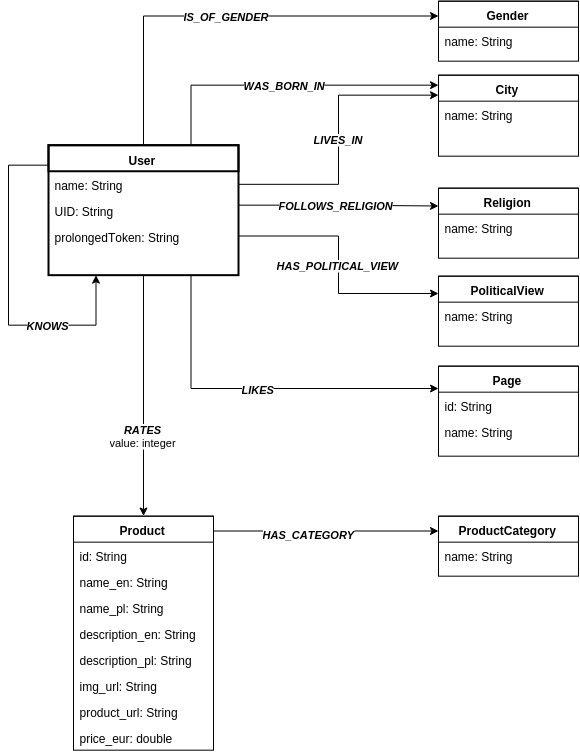
\includegraphics[width=\textwidth]{neo4j_data_model3.png} 
% width=\textwidth
\caption[Data model in Neo4j.]{Data model in Neo4j.}
\label{fig.data_model}
\end{figure}

\subsection{Data constructs}

The Property Graph data model provides four main building blocks for storing data in Neo4j \cite{learning_neo4j}:
\begin{itemize}
\item {\bf Nodes}: store entity information.
\item {\bf Relationships}: connect nodes to one another; they always have a type, a start and an end node, and a direction.
\item {\bf Properties}: key-value pairs belonging to a node / relationship, describing its features.
\item {\bf Labels}: describe the "type" of a node.
\end{itemize}

\subsection{Modelling}

To start modelling a graph database, it is useful to employ an Entity-Relationship diagram, as in the case of relational systems \cite{learning_neo4j}. Next, the following information can be extracted from a domain description:
\begin{itemize}
\item entities -- from the nouns of the description
\item properties -- from the adjectives of the description
\item relationship -- from the verbs in the description
\end{itemize}

[TODO? przykład ER diagram, pokazanie że w GDB nie trzeba join tables? \cite{learning_neo4j}, pp. 77-79]

[TODO? opisanie dobrych/złych praktyk modelowania? (\cite{learning_neo4j}, pp. 79-88)]

\subsection{Reco4Social model}

The data model implemented in the project is presented in Figure \ref{fig.data_model}. The rectangles represent nodes, with labels in bold and properties below. Arrows linking nodes are the relationships, with the relationship types in bold and with optional properties.

The node central to the model is the \texttt{User} node which can be related to almost all other nodes, including itself. The nodes \texttt{Gender}, \texttt{City}, \texttt{Religion}, \texttt{Political\-View} and \texttt{Page} represent user data gathered from his/her Facebook profile. As it can be seen, there are two relationships between \texttt{User} and \texttt{City}, which is perfectly acceptable in graph databases. The \texttt{KNOWS} relationship is self-referencing: it joins two nodes of the same type, in this case it shows that two users are friends on Facebook. Both \texttt{(User)-[LIKES]-(Page)} and \texttt{(User)-[KNOWS]-(User)} are one-to-many relations, while the rest of the above are (but do not have to be) one-to-one relations.

In the lower part of the schema there is the \texttt{Product} node. It belongs to a \texttt{Product\-Category} and can also be linked with a user, when he/she rates the product. The rating value is stored as a property of the \texttt{RATES} relationship. 

[TODO? coś jeszcze?]

\section{Recommendation algorithm}

% - niektórzy użytkownicy nie podali danych społ., albo zalogowali się, po czym zrezygnowali nie oceniwszy żadnego produktu -- należało takich użytkowników odfiltrować przed testami

\begin{figure}
\centering
\includegraphics[width=\textwidth]{recommendation_flow.png} 
\caption[Recommendation flow.]{Recommendation flow. [TODO? Potencjalnie poprawić?]}
\label{fig.recommendation_flow}
\end{figure}

The visual flowchart for the algorithm is presented in Figure \ref{fig.recommendation_flow}. It is based on a kNN (k Nearest Neighbours) Collaborative Filtering algorithm, however the neighbourhood selection process is different. Classically the neighbours are chosen on the basis of similarity to the active user in terms of past ratings of items. Yet in this case the active user has not rated any item, since the RS is designed to serve new users. Instead, the nearest neighbours will be chosen on the basis of their social profile similarity to the active user.

\subsection{Neighbourhood selection}

In order to calculate user similarity, each property of the user's social profile, represented as a relationship between nodes in the database, has been attributed a weight. If two users share the same property, their similarity will be increased by the weight. The exact values are illustrated in Table \ref{table.weights}.

% \vspace{1cm}
% %Simplest working example
% \begin{center}
% \begin{tabular}{ c c c }
%   cell1 & cell2 & cell3 \\ 
%   cell4 & cell5 & cell6 \\  
%   cell7 & cell8 & cell9    
% \end{tabular}
% \end{center}


\begin{table}[!h]
\centering
\caption{Relationship weights.}
\label{table.weights}
\vspace{3mm}
\begin{tabular}{ll}
\hline
Relationship         & Weight \vspace{2mm} \\ \hline
\texttt{LIVES\_IN}            & 3      \\ 
\texttt{WAS\_BORN\_IN}        & 3      \\
\texttt{FOLLOWS\_RELIGION}    & 5      \\
\texttt{HAS\_POLITICAL\_VIEW} & 5      \\
\texttt{IS\_OF\_GENDER}       & 10     \\
\texttt{LIKES}                & 1      \\
\texttt{KNOWS}                & 1      \vspace{2mm} \\
\texttt{ARE\_FRIENDS}         & 20     \vspace{2mm} \\ \hline
\end{tabular}
\end{table}

The weights have been chosen arbitrarily, according to the author's subjective feel of importance of each parameter. For instance the relationship \texttt{ARE\_FRIENDS}, meaning the two users are friends on Facebook, seems the most important, hence a high weight. On the other hand there can be multiple Facebook pages common between two users, thus the \texttt{LIKES} weight is small, as it can be multiplied. [TODO poprawić to, niezgrabne]

To find the common relationships between the active user and others, the Cypher query presented in Listing \ref{listing.cypher_users_common} was used. The \texttt{\{active\-User\}} is replaced in the code with the appropriate \texttt{User} object. Because all user relationships in the data model, apart from \texttt{RATES}, represent his social profile, the query omits this one irrelevant relationship.

\begin{listing}
\begin{minted}[framesep=3mm,fontsize=\footnotesize,bgcolor=gray!20]{psql}
MATCH (m:User)-[r1]-(k)-[r2]-(n:User)
WHERE m={activeUser} AND NOT type(r1)="RATES" AND type(r1)=type(r2) 
RETURN n.UID AS userId, type(r1) AS relType
\end{minted}
\caption{Cypher query for finding the common relationships between the active user and others.}
\label{listing.cypher_users_common}
\end{listing}

In order to find all those that the active user is friends with, a different query is needed, presented in Listing \ref{listing.cypher_users_friends}. To differentiate between the situation where two users have common friends (\texttt{KNOWS}) the query will return a new, fake type of relationship -- \texttt{ARE\_FRIENDS} -- just for the purpose of user similarity evaluation.

\begin{listing}
\begin{minted}[framesep=3mm,fontsize=\footnotesize,bgcolor=gray!20]{psql}
MATCH (m:User)-[r]-(n:User)
WHERE m={activeUser} AND type(r)="KNOWS"
RETURN n.UID AS userId, "ARE_FRIENDS" AS relType
\end{minted}
\caption{Cypher query for finding friends of the active user.}
\label{listing.cypher_users_friends}
\end{listing}

The result of the two queries is a list of key-value pairs of user IDs and relationship types. It is worth noting that the actual node to which a relationship points is not important at all. For instance, the system does not care what the item that both users like is -- the only information that matters is the type of the relationship (in this case: \texttt{LIKES}) and the similarity weight value that this entails.

\hbox{}
The next step is to sum the weights of all common relationships with each user. To illustrate this, let us investigate a simple example. Table \ref{table.sample_rels} shows a sample output of the above Cypher queries. There are two users similar to the active user, with IDs "1" and "2". The relationships common with the active user are listed in the "relType" column. To calculate the similarities, we refer to Table \ref{table.weights} for weights and sum them up for each user. This yields:

\mint[fontsize=\footnotesize]{vim}|User 1: ARE_FRIENDS[20] + WAS_BORN_IN[3] + IS_OF_GENDER[10] + LIKES[1] = 34|

\mint[fontsize=\footnotesize]{vim}|User 2: ARE_FRIENDS[20] + KNOWS[1] + KNOWS[1] + LIKES[1] = 23|

Therefore we conclude that, with respect to the active user, User 1 has the similarity value of 34, which makes him a closer neighbour than User 2 with similarity value of 23.

\begin{table}[!h]
\centering
\caption{Sample common relationships.}
\label{table.sample_rels}
\vspace{3mm}
\begin{tabular}{ll}
\hline
userId         & relType \vspace{2mm} \\ \hline
1       & \texttt{ARE\_FRIENDS}                  \\ 
1       & \texttt{WAS\_BORN\_IN}              \\
1       & \texttt{IS\_OF\_GENDER}       \\
1       & \texttt{LIKES}      \\
2       & \texttt{ARE\_FRIENDS}          \\
2       & \texttt{KNOWS}       \\
2       & \texttt{KNOWS}            \\
2       & \texttt{LIKES}              \vspace{2mm} \\ \hline
\end{tabular}
\end{table}

Finally, when all similarity values have been calculated, the users are sorted descendingly with respect to those values and K users at the top of the list are selected for the products recommendation (K nearest neighbours).

\subsection{Products recommendation}

Having the list of K similar users, for each one their highest rated products are chosen. The definition of what counts as "highly rated" is ambiguous, therefore a~variable \texttt{ratingLowest} has been introduced. As the name suggests, it defines a~threshold -- only products rated by a neighbour equally or higher will be considered for recommendation. The products selected from each neighbour are scanned and added to a global collection, each time preserving the rating and neighbour's similarity to the active user.

Another filtering parameter is \texttt{minNumOfRatings}, which defines how many of the neighbours had to highly rate a product before it can be recommended. It has been introduced to enable control of suggesting unpopular items. 

Next, all remaining products are subjected to suggested rating computation. This is the system's evaluation of how it "thinks" the active user would rate these items. To account for neighbourhood similarity the RS calculates a weighted average of each product's ratings and corresponding user similarity values. The formula is presented in Equation \ref{eq.ratings_weighted}, with the $sim(u,u')$ representing the similarity value between the active user $u$ and a neighbour $u'$ belonging to the set of neighbours $U$, and the $r_{u'i}$ being the neighbour's rating of item $i$.

\begin{equation}
\hat{r}_{ui} = \frac{1}{\displaystyle\sum_{u' \in U} |sim(u,u')|} \left(\displaystyle\sum_{u' \in U} sim(u,u')\cdot r_{u'i}\right)
\label{eq.ratings_weighted}
\end{equation}

In the end the obtained predictions are rounded to integer values, sorted in a descending order and returned in a collection to the module that initiated the process (the recommendation controller or the recommendations validator).







\section{Product selection and user data gathering}
The goal of the product catalog presented to the users was on the one hand to be diverse enough so that everyone could find something that suits them, but on the other hand to be concise enough so the data for the recommender system would not be too scarce.

To balance these two requirements the products could not have been obtained by simply crawling web stores with an automated program, but instead they had to be hand-picked. Most of the products come from Amazon, but also from other existing e-commerce websites. They have been divided in 15 categories, with around 20 products in each category. The obligatory information about each product includes the name and the URL of an image. In some cases other data has also been collected, such as description, price and the URL of the offer.

The test users for the application were recruited among my friends on Facebook. In the end 107 users have logged in to Reco4Social. Unfortunately some of them either blocked access to their social profile information or did not complete the survey. They had to filtered out in order not to obstruct the results. In the end the user base consisted of 90 users.

\section{Web application and social login}
\subsection{Design}

The web application consists of 3 main parts:
\begin{itemize}
\item the login screen
\item the survey - used in the first stage to gather user ratings for products
\item the recommender - used in the second stage to provide recommendations
\end{itemize}

\subsubsection{The login}

\begin{figure}[!h]
\centering
\includegraphics[width=\textwidth]{login_flow.png} 
\caption[Login flow.]{Login flow [TODO poprawić ten schemat].}
\label{fig.login_flow}
\end{figure}

Upon entering the website, the user is presented with the login screen, shown in Figure \ref{fig.login}. The top panel contains two buttons: "About", which opens up a popup with additional information on the project, and "Report problem", which leads to a form created in Google Forms for submitting any issues with the application.

The central panel contains the login button for Facebook. When clicked, it uses the Facebook Javascript API to open a new window and guide the user through the Facebook authentication process. The user needs to authorize the Facebook application to access their data, as depicted in Figure \ref{fig.login.fb_app_auth}. Once that is completed, the window is closed and a callback to the original page is activated, informing about a successful login.

Depending on the stage of the project, the user is then redirected either to the survey or to the recommendation page. 

\begin{figure}[!t]
\centering
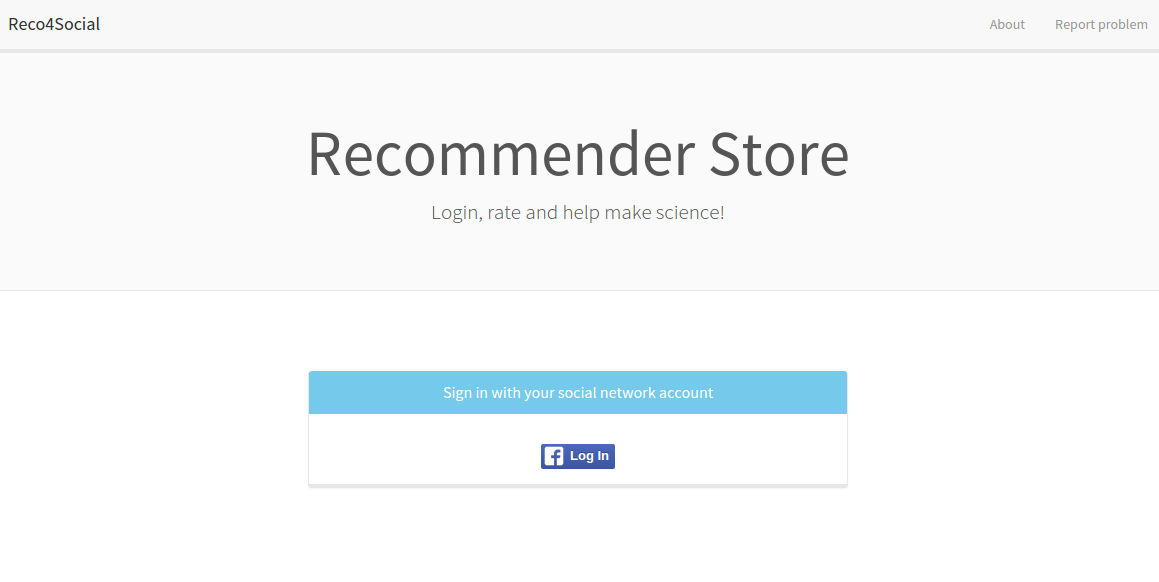
\includegraphics[width=\textwidth]{reco4_login.png} 
\caption[Login page.]{Login page.}
\label{fig.login}
\end{figure}

\begin{figure}[!t]
\centering
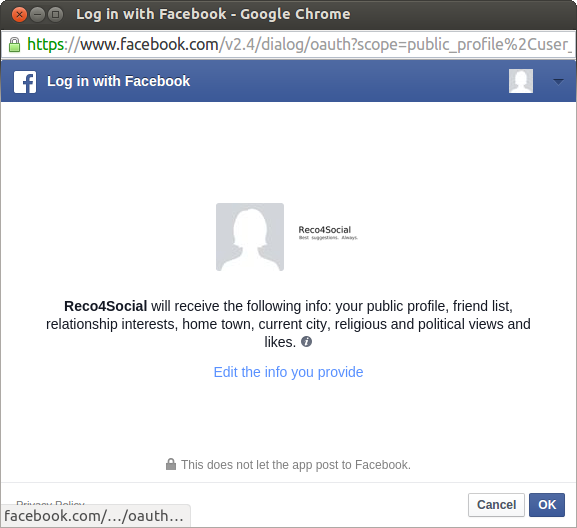
\includegraphics[width=10cm]{fb_auth.png} 
% width=7cm | \textwidth
\caption[Authorizing the Facebook application.]{Authorizing the Facebook application.}
\label{fig.login.fb_app_auth}
\end{figure}

In the background, a Spring component uses the user credentials to query Facebook for additional data. The requested data includes:
\begin{itemize}
\item gender
\item hometown
\item current city
\item political view
\item religion
\item likes - the Facebook pages that the user "likes"
\item friends - only those who have also logged in to my website
\end{itemize}

If during the application authorization process the user edited the sharing options, some or all of the above data may not be accessible.

The received information is processed in the background and stored in the graph database.

\subsubsection{The survey}
\begin{figure}[!t]
\centering
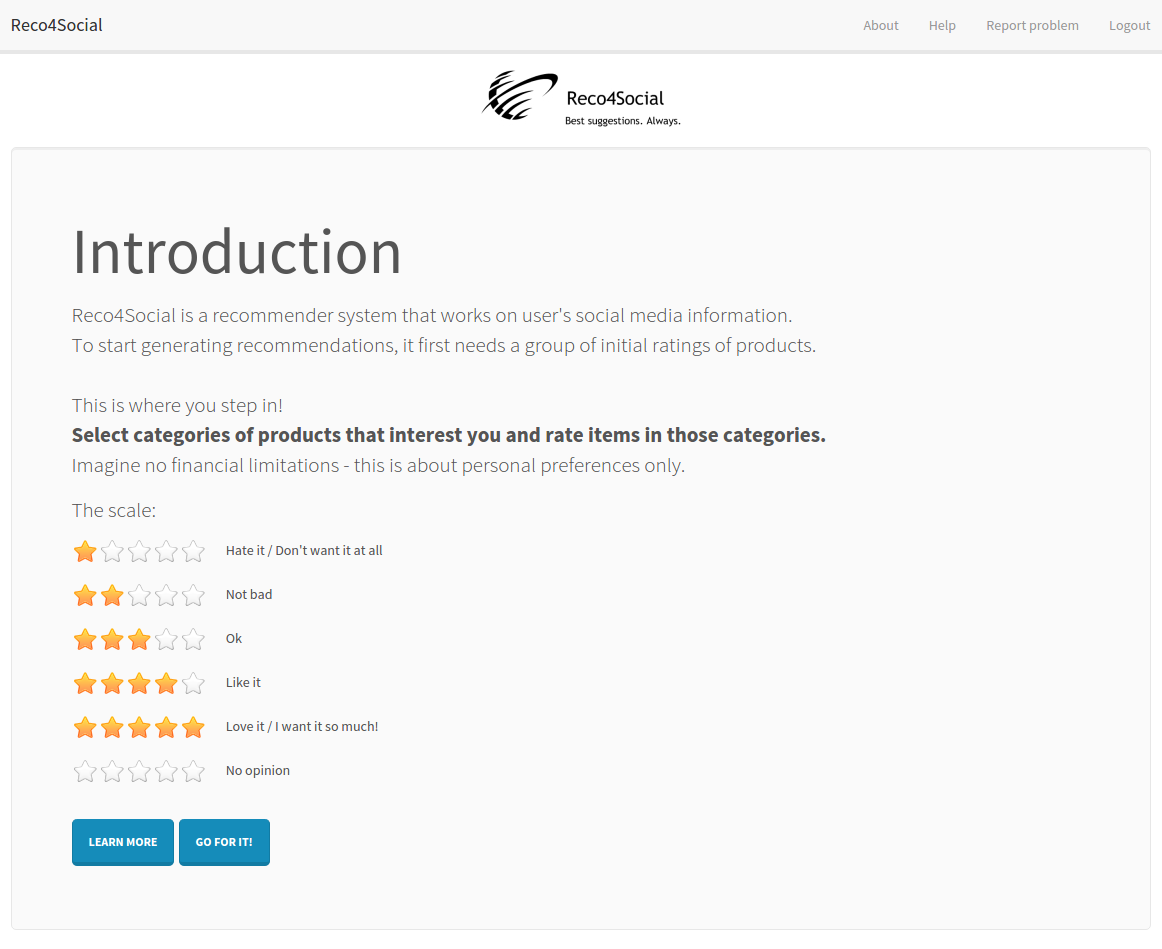
\includegraphics[width=\textwidth]{reco4_survey-intro-1.png} 
\caption[Survey introduction.]{Survey introduction.}
\label{fig.survey.intro-1}
\end{figure}

\begin{figure}[!t]
\centering
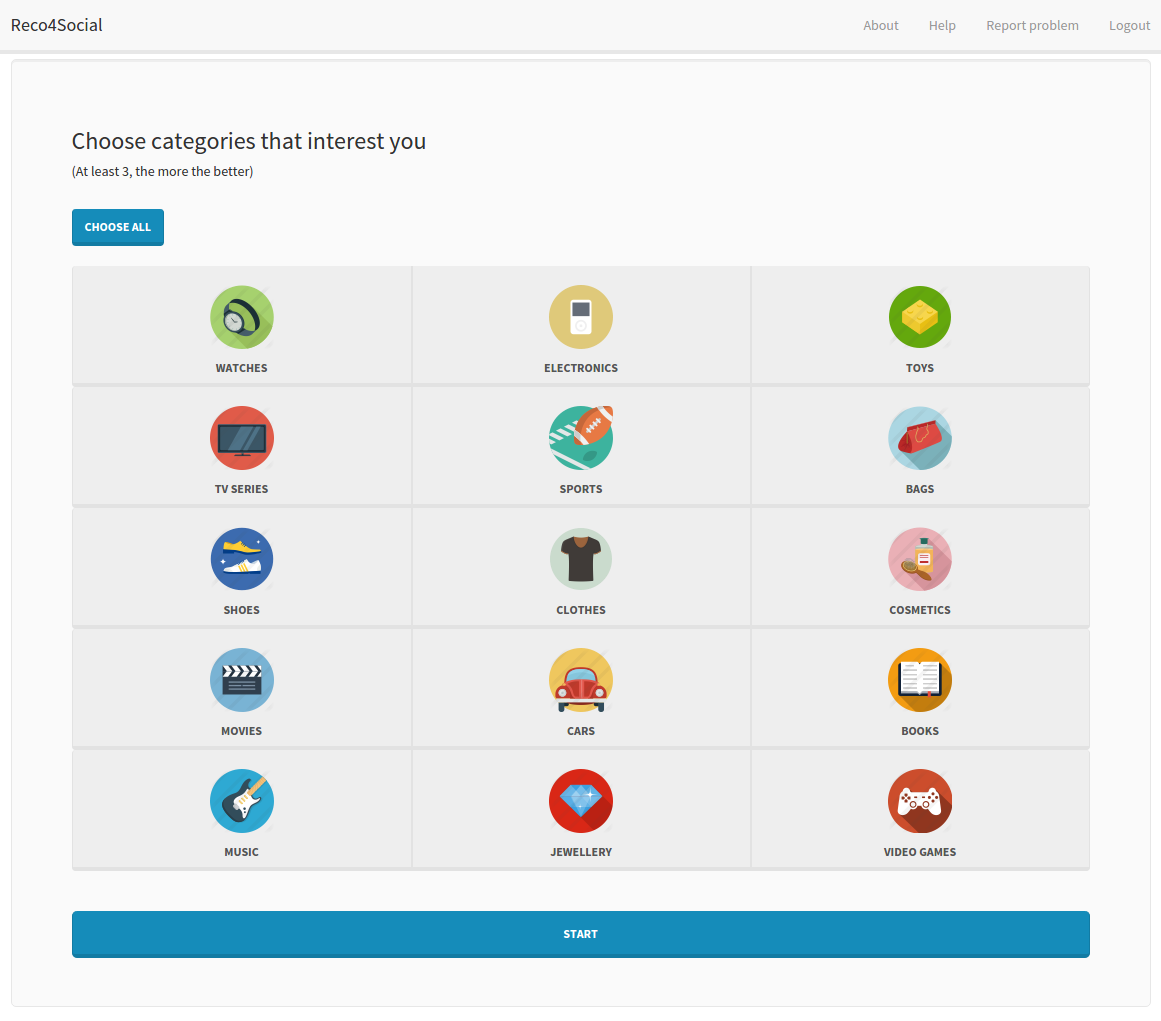
\includegraphics[width=\textwidth]{reco4_survey-intro-2.png} 
\caption[Survey product categories selection.]{Survey product categories selection.}
\label{fig.survey.intro-2}
\end{figure}

\begin{figure}[!t]
\centering
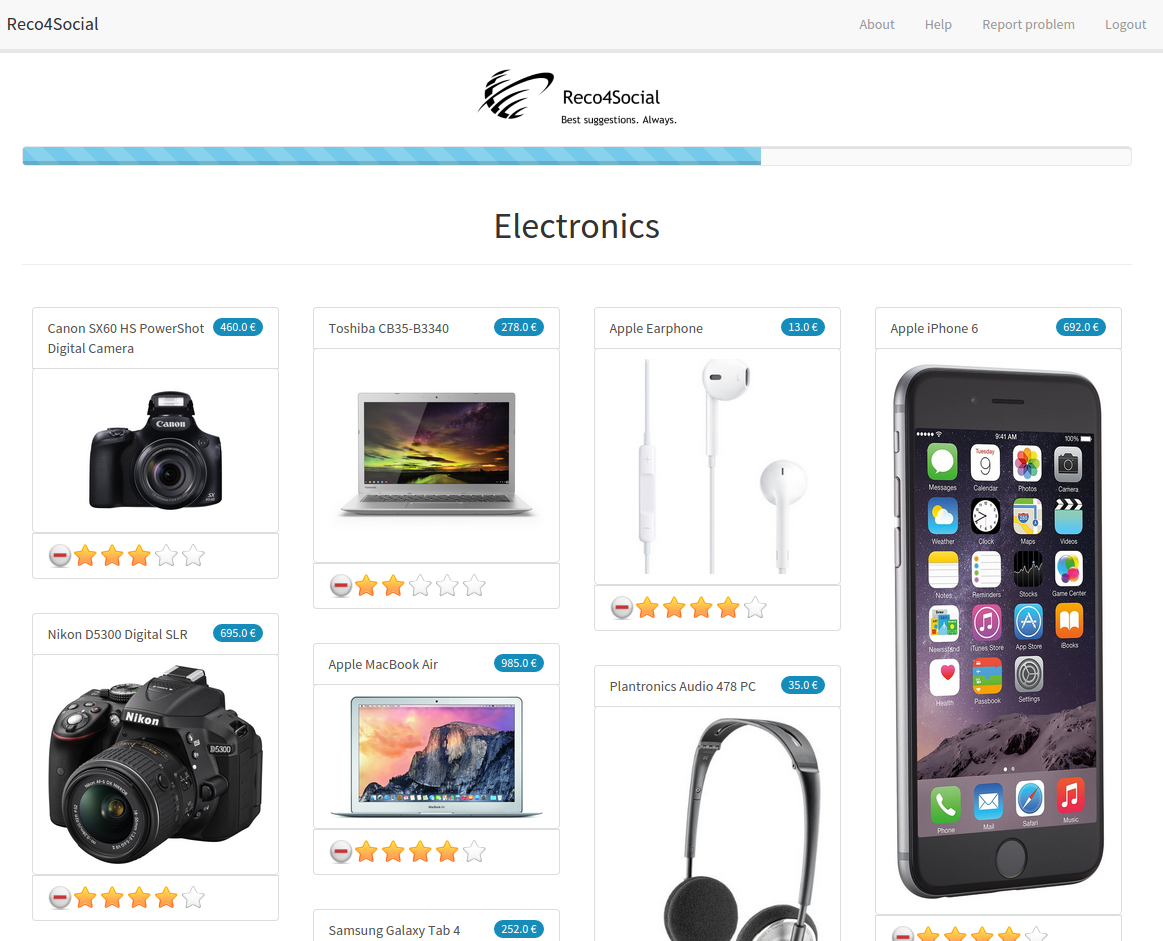
\includegraphics[width=\textwidth]{survey2.png} 
\caption[The survey.]{The survey.}
\label{fig.survey}
\end{figure}

\begin{figure}[!t]
\centering
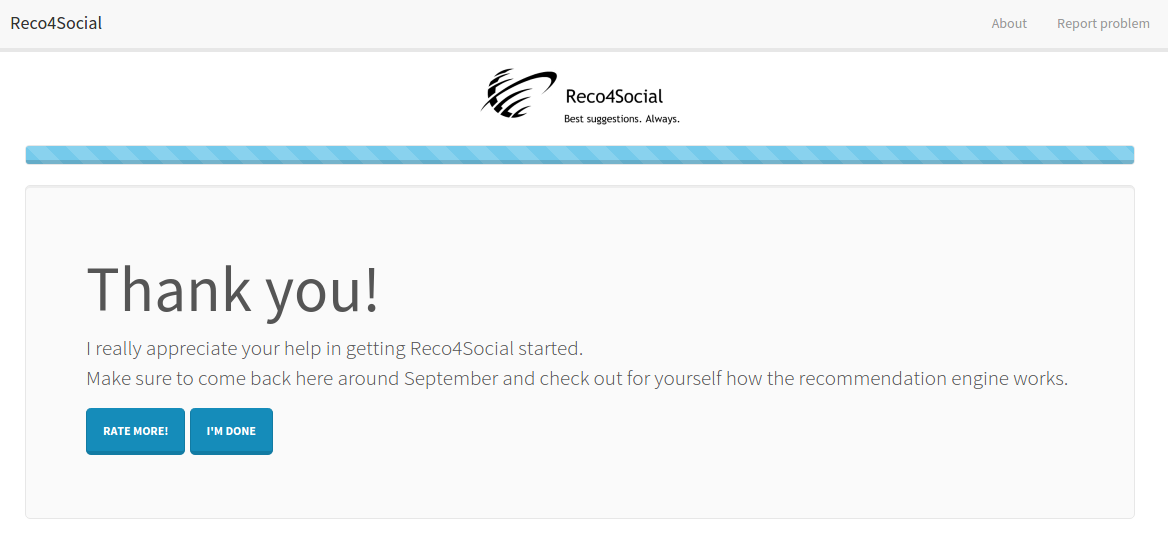
\includegraphics[width=\textwidth]{survey_end.png} 
\caption[The survey end.]{The survey end.}
\label{fig.survey.end}
\end{figure}

After having successfully logged in, the user is presented with an introduction to the survey, visible in Figure \ref{fig.survey.intro-1}. It explains what the project is about and how to complete the survey, including the description of the rating system.

Users are supposed to choose categories of products that interest them (at least three) and then to rate products in those categories according to their tastes. The rating scale is 1-5, where 1 means "do not like at all" and 5 means "love it". If a user has no opinion about a particular product, they are supposed to leave the rating empty.

For those users that seek additional information about the project, there is the "Learn more" button, which opens a popup window with a more detailed explanation.

Figure \ref{fig.survey.intro-2} shows the categories selection panel, which is located just below the introduction. The users are asked to choose at least three categories, otherwise they are not permitted to proceed. The "Start" button redirects the user to the actual survey.

The survey page (Figure \ref{fig.survey}) presents all products from each category, one at a time. At the top a progress bar informs the user how many categories are left. Each product is contained within a "box", displaying the item's name, picture, price and the rating to be filled. The rating is presented in the form of "stars".

A button at the bottom reloads the page presenting products from the next category. In the case of the last category, it redirects to the survey end page. It is shown in Figure \ref{fig.survey.end} and contains the acknowledgement of the user's contribution to the project.

\subsubsection{The recommender}

% In the second stage of the project, with the initial user base ready, a new visitor is presented with the recommendations page after login.

% In the second part of the project, when a user has logged in with Facebook, he/she is no longer redirected to the survey, but instead is presented with 
In the second stage of the project, with the initial user base ready, a new visitor is presented with the main store page after login. The centerpiece of the page is the recommendations pane. In a real life situation this would be a typical storefront, with the "suggested items" block located on top of the page or somewhere to the side.

One of the design goals was to make the recommender seamlessly integrate with any existing storefront. Even though the RS generates recommendations very quickly, within the time frame of a web request and response, the limiting factor is the social network user data fetching, which takes up a significant amount of time (several seconds, depending on the user). Moreover, if the system were to serve more users, the RS could operate slightly longer (though the impact would be much lower than in the case of a relational database).

With that in mind, the recommendations presentation was designed to be asynchronous. When the store's main page has loaded, an AJAX request is sent to the controller. It then repeatedly checks whether user data fetching has finished. When it is done the controller starts the RS and then sends its results back to the view (the web page). 

[TODO może to trochę zmienimy, żeby to nie kontroler inicjował RS tylko jednak ten FBservice. W ten sposób rekomendacje nie będą "przekalkulowywane" ponownie przy każdym załadowaniu strony.]

As soon as the AJAX request has been sent, the user is presented with a "Generating recommendations..." loading image. When the backend processing has finished and an AJAX response is received, the image is replaced with the generated recommendations. This process is illustrated in Figure \ref{fig.reco_gen_done}.

\begin{figure}[!t]
\centering
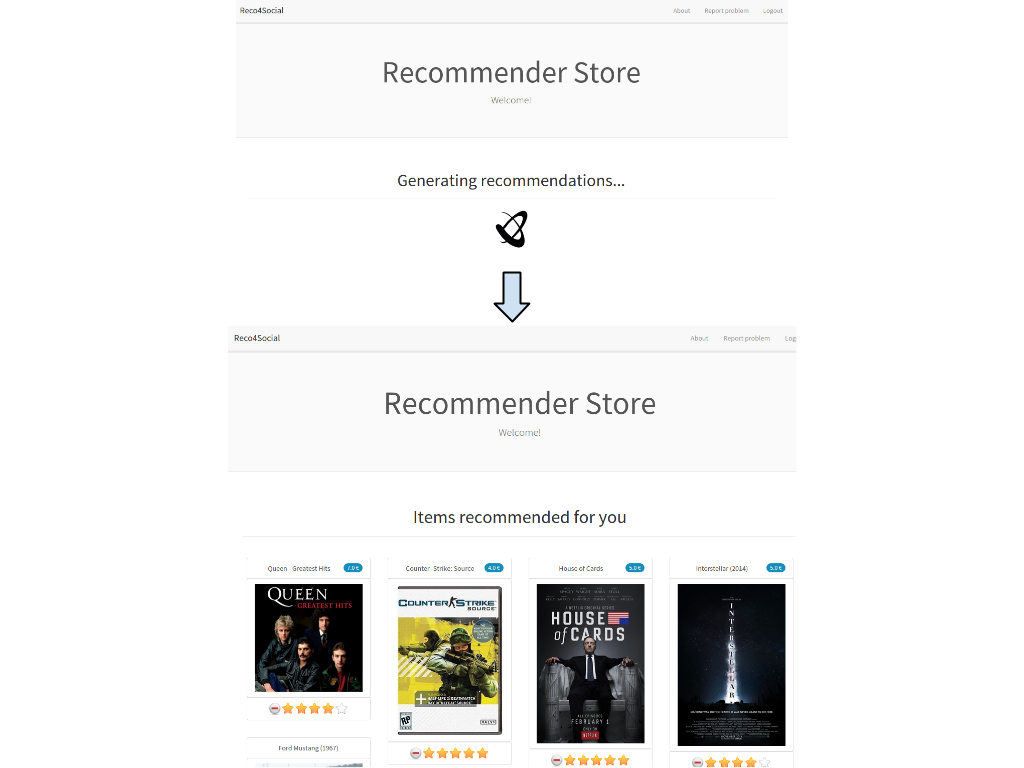
\includegraphics[width=\textwidth]{reco_gen_done.png} 
\caption[Recommendations generation.]{Recommendations generation. [TODO zmienić to? większy obrazek z lepszą rozdzielczością?]}
\label{fig.reco_gen_done}
\end{figure}

\hbox{}
Thanks to this approach the RS processing does not slow down page loading and would not in any way hamper the user's experience with a real store. This is crucial nowadays, as page loading time is one of the key factors for users, which tend to abandon sites that load too slowly.

\subsection{Facebook application configuration}
The first step in using the Facebook API is application creation. User data can only be accessed when they grant the appropriate privileges to our application.

The place for managing Facebook applications is the Developer center, available at the URL: \url{https://developers.facebook.com/}.

To properly configure a new App, multiple details need to be provided, including the name, category, type (iOS, Android, web), its domain, website etc. Afterwards, two parameters are generated: App ID and App Secret, that allow client authorization.

When new App is created, at first it possesses only the basic permissions for accessing users' data, namely the \url{public_profile}, \url{email} and \url{user_friends} items.

In order to gain permissions for additional information, an approval submission needs to be filled in. Facebook expects detailed explanation, along with screenshots of the website, of how the obtained data will be used. At first my submission was rejected, however the second time, after having underlined that my project is not commercial, but purely academic, the permissions were granted.

In the end the Facebook App has the following permissions that are used in the project:
\begin{itemize}
\item \url{public_profile}
\item \url{user_friends}
\item \url{user_hometown}
\item \url{user_location}
\item \url{user_religion_politics}
\item \url{user_likes}
\end{itemize}

[TODO Graph API? Na jakie EP uderzamy? czy to dalej?]

\subsection{Implementation}

The web application is created with the MVC design pattern in mind. Therefore a \textit{Model} manages the data and logic of the application, a \textit{View} presents data to the user in the form of HTML documents and a \textit{Controller} acts as an intermediary between the two, sending data from a model to a view as well as gathering user input from the view and transmitting the information back to the model.

The project structure is typical for Spring, with the following main folders under \texttt{/src/main}:
\begin{itemize}
\item \texttt{java} contains all Java classes, divided into packages:
    \begin{itemize}
    \item \texttt{controllers}: Controller classes
    \item \texttt{facebook}: \texttt{FacebookService} responsible for accessing Facebook data.
    \item \texttt{labels}: \texttt{Label} interface implementations for Neo4j nodes.
    \item \texttt{neo4j}: Classes accessing the database.
    \item \texttt{prop}: Properties classes.
    \item \texttt{recommender}: Classes generating and validating recommendations.
    \end{itemize}
\item \texttt{resources} contains \texttt{properties} files.
\item \texttt{webapp} contains views (JSP files) and JS/CSS files.
\end{itemize}


\subsubsection{The login}

The view containing the login page layout is \texttt{login.jsp}. It defines the layout with the use of HTML and by importing the appropriate CSS files. Some elements that are repeatable on many pages, such as the navigation bar or the footer, are defined in their own JSP files and included where necessary (an example is shown in Listing \ref{listing.jsp_include}).

% frame=lines,
\begin{listing}
\inputminted[framesep=3mm,fontsize=\footnotesize,bgcolor=gray!20]{jsp}{code_jsp_include.jsp}
\caption{Example of including repeatable JSP elements from files.}
\label{listing.jsp_include}
\end{listing}

All JSPs also import JavaScript libraries and can define their own JS code. In the case of \texttt{login.jsp}, it contains all methods necessary to connect to Facebook for user authentication and authorisation. They are based on exemplary code available on the Facebook Developers page \cite{facebook_login_web}.

In order to allow the users to log in, a Login Button social plugin was included. It is a custom HTML5 element that triggers the Facebook JavaScript SDK \texttt{login()} method when clicked. It accepts additional data as attributes of the HTML element. One of them is \texttt{scope}, where all permissions required from each user are defined. It is on this basis that this information can then be accessed from a user's profile. The login button declaration is depicted in Listing \ref{listing.login_button}.

\begin{listing}
\inputminted[framesep=3mm,fontsize=\footnotesize,bgcolor=gray!20]{html}{code_login_button.html}
\caption{The Facebook login button declaration.}
\label{listing.login_button}
\end{listing}

Upon successful Facebook login the page form is submitted to the \texttt{Login\-Controller.java}. Method resposible for handling this POST request is \texttt{home\-Submit()} and its simplified version is shown in Listing \ref{listing.controller_login_homesubmit} to illustrate how controllers are built.

\begin{listing}[!t]
\inputminted[framesep=2mm,fontsize=\footnotesize,bgcolor=gray!20]{java}{code_controller_login.java}
\caption{\texttt{LoginController.java} fragment.}
\label{listing.controller_login_homesubmit}
\end{listing}

First, the \texttt{LoginController} class requires the Spring's \texttt{@Controller} annotation above the class name in order to be interpreted as a controller component. The particular method that handles the page submit also has an annotation: \texttt{@Request\-Mapping}. It maps a particular URL, defined as \texttt{value} attribute, to this method -- in this case it is the \texttt{/login} URL. Moreover, by defining the \texttt{method} attribute the scope of this method is limited to handle only POST requests.

The method obtains a \texttt{User} object from the view, containing the \texttt{access\-Token} received from Facebook as a result of authentication. This token is then used each time when connecting to Facebook from the backend. In this case, with the use of RestFB, a lightweight Java library, a \texttt{Default\-Facebook\-Client} object is created. Next, it fetches the user's basic social profile data, available in the Facebook Graph API at the \texttt{/me} URL.

This data is used to create a user node in the database with the use of the \texttt{getUserNode()} method in the \texttt{GDBM} (\texttt{Graph\-DB\-Manager} object). Next, the \texttt{access\-Token} and \texttt{userId} are set as session attributes for future reference. Finally, the \texttt{process\-User} method in the \texttt{Facebook\-Service} component will asynchronously fetch all the remaining user data from the social network and the user is redirected to the store's main page.

\hbox{}
To access objects such as the aforementioned \texttt{GDBM} or \texttt{Facebook\-Service} the Spring's dependency injection mechanism is used. Instead of manually instantiating the objects, one only needs to append the \texttt{@Autowired} annotation to the field declaration, as presented in Listing \ref{listing.autowiring}. However, for this to be possible, the \texttt{app-context.xml} file should contain an XML element \texttt{context:\-component\--scan} configured to indicate packages that Spring should scan for the autowired dependencies.

\begin{listing}
\begin{minted}[framesep=3mm,fontsize=\footnotesize,bgcolor=gray!20]{java}
@Autowired
private FacebookService facebookService;
@Autowired
private GraphDBManager GDBM;
\end{minted}
\caption{Dependency injection in Spring with the \texttt{@Autowired} annotation.}
\label{listing.autowiring}
\end{listing}

[TODO? opisać FacebookService?]

[TODO opisać API Neo4j, jak uzytkownicy i relacje sa tworzone]

\subsubsection{The survey}

Survey introduction is defined in the \texttt{survey\-\_intro\-.jsp} view and is handled by \texttt{Survey\-Intro\-Controller}. The list of all possible product categories is fetched from the model by the controller and passed to the view as an attribute of a \texttt{Model\-Map}, where they are all presented to the user to choose those that interest him/her. 

The user is required to choose at least three categories. There is a front-end validation that, if less categories are selected, will not submit the form and will instead show the user an error message, prompting to rectify the choice. It has been realized with the use of the jQuery Validate plugin \cite{jquery_validate}.

When the user choice is submitted, the controller stores the selected categories in an array in the session and redirects the user to the survey.

\hbox{}
Analogically, the survey page is administered by \texttt{survey\-.jsp} and \texttt{Survey\-Controller}. The products presentation has been implemented on the basis of an online e-commerce template \cite{bootply_ecommerce}. The "star" rating system was developed using the jQuery Raty plugin \cite{jquery_raty}. Each time a user rates a product, an AJAX POST request is sent to the controller and the rating is stored in the database. This feature has been implemented in order to avoid situations where the user would abandon the survey in the middle of a category and all his ratings for this category would be lost without the form submission.

[TODO? coś jeszcze?]

\subsubsection{The recommender}

The main page of the store is defined in the \texttt{main\-.jsp} view and is handled by the \texttt{HomeController}. When the view has loaded, it requests the controller for recommendations, which in turn initiates the RS.

The class responsible for calculating the similarities is \texttt{User\-Similarity\-Processor}. Listing \ref{listing.find_similar_users} shows the method \texttt{find\-Similar\-Users()} used to find K nearest neighbours of a user. It invokes methods from \texttt{GraphDB\-Manager} which performs relevant queries on the database to find all similarities between the active user and others. The \texttt{process\-Common\-Interests\-Map()} method then sums the weights of all common relationships. Finally the users are sorted descending with similarity and are limited to K nearest neighbours.

\begin{listing}[!h]
\begin{minted}[framesep=3mm,fontsize=\footnotesize,bgcolor=gray!20]{java}
public List<SimilarUser> findSimilarUsers(String userId, int howMany) {
    List<SimilarUser> similarUsersSortedList = new ArrayList<>();
    Map<String, SimilarUser> similarUsersMap = LinkedHashMap<>();

    processCommonInterestsMap(GDBM.getOtherUsersWithRelationship(
        GDBM.getUserNode(userId)), similarUsersMap);
    processCommonInterestsMap(GDBM.getOtherUsersFriendship(
        GDBM.getUserNode(userId)), similarUsersMap);
    similarUsersMap = sortUsersDescendingWithSimilarity(similarUsersMap);

    int counter = 0;
    for(Map.Entry<String, SimilarUser> entry : 
        similarUsersMap.entrySet()) {
        if(counter <= howMany) {
            counter++;
            SimilarUser user = entry.getValue();
            user.userId = entry.getKey();
            similarUsersSortedList.add(user);
        } else break;
    }
    return similarUsersSortedList;
}

public void processCommonInterestsMap(Map<String, Map<String,AtomicInteger>>
    commonInterestsMap, Map<String, SimilarUser> similarUsersMap) {
    commonInterestsMap.forEach((userId, relMap) -> {
        SimilarUser user = createSimilarUserIfNotExistsAndPutIntoMap(
            similarUsersMap, userId);
        relMap.forEach((relName, count) -> {
            double similarityWeight = GraphConstants.similarityWeights.get(
                GraphConstants.RelTypes.valueOf(relName));
            user.similaritySum += similarityWeight * count.intValue();
        });
    });
}
\end{minted}
\caption{Method for finding similar users.}
\label{listing.find_similar_users}
\end{listing}

With that data the \texttt{ProductRecommender} component starts generating recommendations according to the algorithm. When finished, the list of products with suggested ratings is sent back to the view via the controller and shown to the active user.

%


\chapter{Evaluation}

[TODO jakiś wstęp]

- jak zostala zrobiona (idea, że offline, k-fold x-valid. etc.)

- że z ponad 100 userów zrobiło się 90 po odfiltrowaniu

\section{Evaluation of predictive and classification accuracy}

\subsection{Ratings prediction accuracy}

Prediction accuracy is the most popular metric in the recommendation system literature \cite{eval_microsoft}. It defines how correct the recommendation results are compared to real user data. 
% For this a test user base with ratings is needed. 

There are two main measures of prediction accuracy which were used in testing Reco4Social:
\begin{itemize}
\item {\bf Root Mean Squared Error (RMSE)}: The system generates predicted ratings $\hat{r}_{ui}$ for a test set $N$ of user-item pairs $(u,i)$ for which the true ratings $r_{ui}$ are known. In this case the ratings were obtained from users during the initial, survey part of the project. The formula for calculating the RMSE between the predicted and actual ratings is:
\end{itemize}

\begin{equation}
RMSE = \sqrt{\frac{1}{|N|} \displaystyle\sum_{(u,i) \in N} (\hat{r}_{ui} - r_{ui})^2 }
\label{eq.rmse}
\end{equation}
\hbox{}

\begin{itemize}
\item {\bf Mean Absolute Error (MAE)}: This is a similar alternative, given by the formula:
\end{itemize}

\begin{equation}
MAE = \frac{1}{|N|} \displaystyle\sum_{(u,i) \in N} |\hat{r}_{ui} - r_{ui}|
\label{eq.mae}
\end{equation}
\hbox{}

Both RMSE and MAE describe the error in the same units as the computed values, i.e. and RMSE=1 means that on average the system's predicted rating was off by 1 with respect to the real rating. Moreover, RMSE uses the squared deviations and thus emphasises larger errors in comparison to MAE.

\subsection{Classification accuracy}

This is an accuracy metrics that measures how well the system can classify items as relevant or not \cite{eval_twente}. The magnitude of the error between the predicted and real rating is ignored.

There are two dominant measures, precision and recall. {\bf Precision} is the ratio of relevant items selected to the number of all selected items. It would be easy to recommend many items and count on the fact that some of them might interest the user. The goal is, however, to show only the important items. The higher the precision, the better the RS in this regard. The formula for precision calculation is presented in Equation \ref{eq.precision}, where $B_{rs}$ represents the relevant selected items and $B_s$ stands for all the selected items.

\begin{equation}
Precision = \frac{|B_{rs}|}{|B_{s}|}
\label{eq.precision}
\end{equation}
\hbox{}

{\bf Recall}, on the other hand, represents the ratio between the number of relevant items selected and the total number of relevant items $B_r$. It illustrates how many of all items interesting to the user was the system capable of finding. Equation \ref{eq.recall} shows the formula for recall calculation.

\begin{equation}
Recall = \frac{|B_{rs}|}{|B_{r}|}
\label{eq.recall}
\end{equation}
\hbox{}

In order to find precision and recall, the notion of relevance has to be defined. For the purpose of this evaluation the following approach was used: considering all items rated by the user 4-5 as relevant, and all those rated 1-3 as non relevant. The items that were not rated at all are ignored.
% For the purpose of this evaluation two approaches were employed:
% \begin{itemize}
% \item considering all items rated by the user 4-5 as relevant, and all those rated 1-3 as non relevant
% \item calculating the average rating for each user (for all products) and using it as a threshold -- all items rated below are not relevant and all those rated above are relevant.
% \end{itemize}

It has been shown that precision and recall are related -- when one increases, the other decreases. There exist methods that take both of them into account and produce a single metric. The most popular is the {\bf F-measure}, illustrated in Equation \ref{eq.fmeasure}, which is a harmonic mean of precision and recall. The results are on a scale from 0 (worst) to 1 (best).

\begin{equation}
F_1 = 2\:\frac{Precision \times Recall}{Precision + Recall}
\label{eq.fmeasure}
\end{equation}
\hbox{}

\subsection{Results}

The evaluation was performed by calculating RMSE, MAE, Precision, Recall and F-measure for each user in the database. This approach represents a K-fold cross validation with the active user as a one-element \textit{validation set} and all other users as the \textit{training set}.

Moreover, this process was repeated for varying values of \texttt{K} and \texttt{minNumOf\-Ratings} -- both in the range from 1 to 10. The \texttt{ratingLowest} has been set to 4 as the threshold for relevancy.

The detailed test results can be found in Appendix 1 [TODO? tak, czy dać tylko tu wybrane i już?] and the selected best results are presented in Table \ref{table.results}.

\begin{table}[!h]
\centering
\caption{Selected test results.}
\label{table.results}
\vspace{3mm}
\begin{tabular}{|l|l|l|l|l|l|l|}
\hline
K  & minNumOfRatings  & RMSE         & MAE          & Recall       & Precision    & F-measure     \\ \hline
4  & 4  & {\bf 0.7842} & {\bf 0.6007} & 0.0736       & 0.3229       & 0.1087       \\ \hline
6  & 5  & {\bf 0.7716} & {\bf 0.5911} & 0.0680       & 0.3535       & 0.1005       \\ \hline
8  & 3  & 1.5215       & 1.1414       & 0.4704       & 0.2669       & {\bf 0.3068} \\ \hline
10 & 1  & 1.8199       & 1.4280       & {\bf 0.9006} & 0.1617       & 0.2602       \\ \hline
10 & 3  & 1.5696       & 1.1825       & 0.5568       & 0.2502       & {\bf 0.3165} \\ \hline
10 & 6  & 1.0631       & 0.8216       & 0.1342       & {\bf 0.3564} & 0.1651       \\ \hline
\end{tabular}
\end{table}

The general trend of how the parameters vary within a constant \texttt{K} and a changing \texttt{minNumOfRatings} is depicted in Figure \ref{fig.results_chart_k-8} for \texttt{K}=8.

\begin{figure}[!h]
\centering
\includegraphics[width=\textwidth]{results_chart_k-8.png} 
\caption[Results for K=8.]{Results for K=8.}
\label{fig.results_chart_k-8}
\end{figure}

\section{Evaluation of computation time and resource consumption}
\section{Comparison to non-social recommender systems}

\chapter{Summary and conclusions}
\section{Conclusions}
\section{Usability of the project in AMG.net/Atos}
\section{Future development perspectives}

- większy zbiór użytkowników i produktów --> dłuższe wyliczanie rekomendacji. może jakieś optymalizacje?\\

- przechowywanie raz wyliczonych rekomendacji w bazie, jakies batch-owe przeliczanie

- podpięcie do klasycznego CF
-- wpływ innych czynników na rozwój rekomendacji: interakcja ze stroną, przeglądanie produktów etc.

- avoid supernodes (the dense node pattern, \cite{learning_neo4j}, pp. 88-89)

% \chapter{Bibliography}

% \chapter{Appendices}

\addcontentsline{toc}{chapter}{Bibliography} 
\begin{thebibliography}{99}

\bibitem{rise_of_social_commerce}
Lora Cecere, \textit{Rise of Social Commerce}, Altimeter Group conference presentation, 2010, Available at: \url{http://www.riseofsocialcommerce.com/wp-content/uploads/2010/10/Lora_Cecere-Rise_of_Social_Commerce.pdf}, [access: 1 May 2015].

\bibitem{snrs}
Jianming He, Wesley W. Chu, \textit{A Social Network-Based Recommender System (SNRS)}, Computer Science Department, University of California, Available at: \url{http://www.cobase.cs.ucla.edu/tech-docs/jmhek/snrs.pdf}, [access: 25 April 2015].

\bibitem{social_login}
Loren McDonald, \textit{Social Login: A Data Capture Game Changer}, Silverpop blog (An IBM Company), 29 November 2011, Available at: \url{http://www.silverpop.com/blogs/email-marketing/social-login-data-capture.html}, [access: 28 August 2015].

\bibitem{spring_framework}
Web page of the \textit{Spring Framework}, Pivotal Software, Available at: \url{http://projects.spring.io/spring-framework/}, [access: 28 August 2015].

\bibitem{lumen}
Web page of a Bootstrap theme, \textit{Lumen}, Available at: \url{https://bootswatch.com/lumen/}, [access: 28 August 2015].

\bibitem{restfb}
Web page of \textit{RestFB}, Available at: \url{http://restfb.com/}, [access: 28 August 2015].

\bibitem{neo4j}
Web page of \textit{Neo4j}, Available at: \url{http://neo4j.com/}, [access: 28 August 2015].

\bibitem{social_commerce_syzygy}
Paul Marsden, \textit{Social Commerce: Monetizing Social Media}, Syzygy Group, 2010, pp. 2-12, Available at: \url{http://digitalintelligencetoday.com/downloads/White_Paper_Social_Commerce_EN.pdf}, [access: 1 September 2015].

\bibitem{rec_sys_handbook}
Francesco Ricci, Lior Rokach and Bracha Shapira, \textit{Introduction to Recommender Systems Handbook}, Recommender Systems Handbook, Springer, 2011, pp. 1-35, Available at: \url{http://www.inf.unibz.it/~ricci/papers/intro-rec-sys-handbook.pdf}, [access: 2 September 2015].

\bibitem{graph_databases}
Ian Robinson, Jim Webber and Emil Eifrem, \textit{Graph Databases}, O'Reilly, 2013, pp. 1-10.

\bibitem{learning_neo4j}
Rik Van Bruggen, \textit{Learning Neo4j}, Packt Publishing, 2014, pp. 11-41:74-[TODO]. Available at: \url{http://neo4j.com/book-learning-neo4j/}, [access: 26 March 2015].

\bibitem{ben_gurion}
David Ben-Shimon et al., \textit{Recommender System from Personal Social Networks}, Ben-Gurion University, Available at: \url{http://fohs.bgu.ac.il/research/upload/23408/RECOMMENDER%20SYSTEMS%20FROM%20SOCIAL%20NETWORK.pdf}, [access: 26 April 2015].

\bibitem{eval_microsoft}
Guy Shani and Asela Gunawardana, \textit{Evaluating Recommendation Systems}, Microsoft Research, pp. 15-16, Available at: \url{http://research.microsoft.com/pubs/115396/EvaluationMetrics.TR.pdf}, [access: 11 May 2015].

\bibitem{eval_twente}
Joost de Wit, \textit{Evaluating Recommender Systems}, TNO Information and Communication Technology, University of Twente, pp. 28-30, Available at: \url{http://essay.utwente.nl/59711/1/MA_thesis_J_de_Wit.pdf}, [access: 11 May 2015].

\bibitem{facebook_login_web}
\textit{Facebook Login for the Web with the JavaScript SDK}, Facebook Developers website, Available at: \url{https://developers.facebook.com/docs/facebook-login/web}, [access: 10 September 2015].

\bibitem{jquery_validate}
Web page of \textit{jQuery Validate} plugin, Available at: \url{http://jqueryvalidation.org/}, [access: 5 May 2015].

\bibitem{bootply_ecommerce}
Web page of an \textit{E-Commerce Template}, Bootply.com, Available at: \url{http://www.bootply.com/s7dUyTggDX}, [access: 5 May 2015].

\bibitem{jquery_raty}
Web page of \textit{jQuery Raty}, Available at: \url{http://wbotelhos.com/raty}, [access: 5 May 2015].

\end{thebibliography}

\addcontentsline{toc}{chapter}{List of figures} 
\listoffigures

\addcontentsline{toc}{chapter}{List of tables} 
\listoftables

\end{document}

